\newpage
\section{Vorbereitungen}
\label{sec:a1}
\subsection{a)}
\label{subsec:a1}
Zu Begin werden die Attribute mit der
höchsten Korrelation zu dem Attribut SalePrice bestimmt.
Diese werden mit dem Prozess Blatt8/Prozesse/Korrelationbestimmen.rmp
bestimmt, die weiteren Aufgaben sind ebenfalls in diesem Prozess zu finden.
\begin{align*}
&\text{1.OverallQual} &:0,790\\
&\text{2.GrLivArea}   &:0,708\\
&\text{3.GarageCars}  &:0,640
\end{align*}
In den Abbildungen \ref{fig:1}-\ref{fig:3} sind die jeweiligen
Korrelation als Scatter-Plot dargestellt.
\begin{figure}
  \centering
  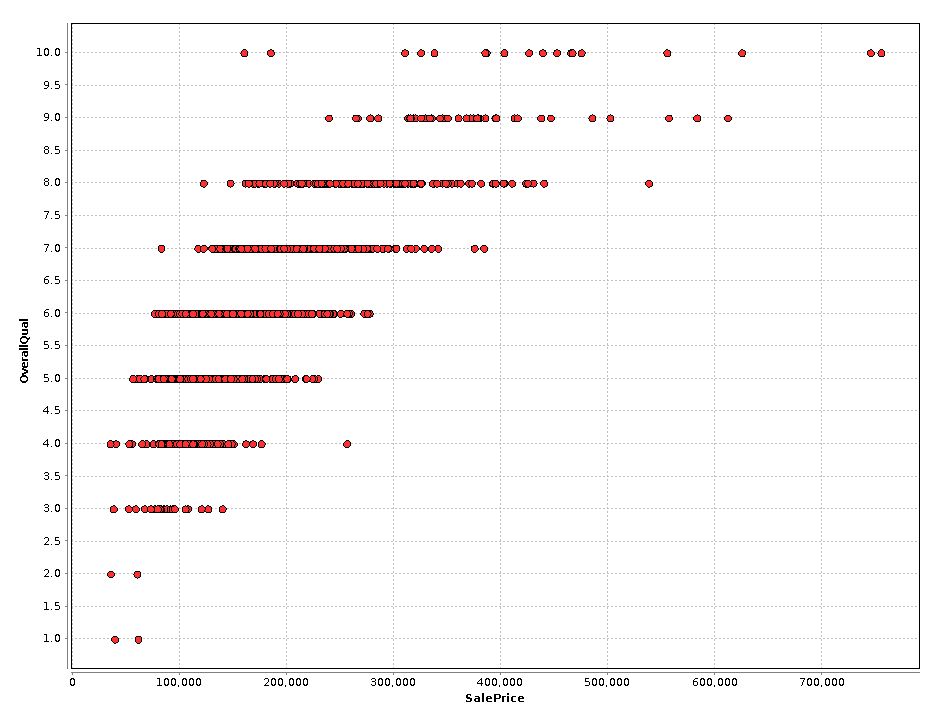
\includegraphics[width=0.7\textwidth]{OverallQual.png}
  \caption{Scatter-Plot von der Korrelation von SalePrice
  und OverallQual.}
  \label{fig:1}
\end{figure}

\begin{figure}
  \centering
  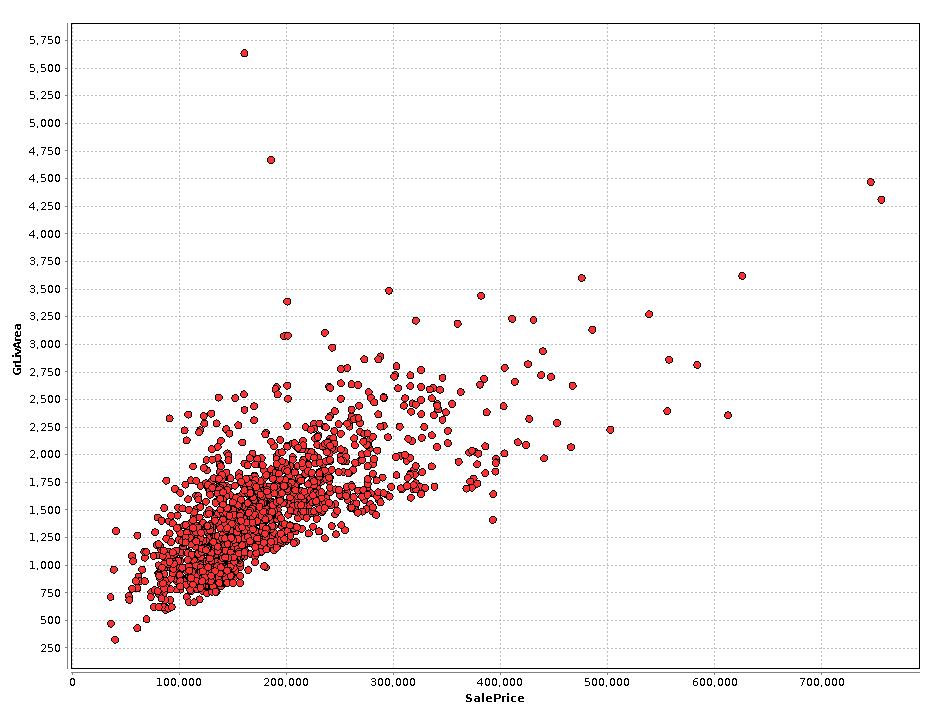
\includegraphics[width=0.7\textwidth]{GrLivArea.png}
  \caption{Scatter-Plot von der Korrelation von SalePrice
  und GrLivArea.}
  \label{fig:2}
\end{figure}


\begin{figure}
  \centering
  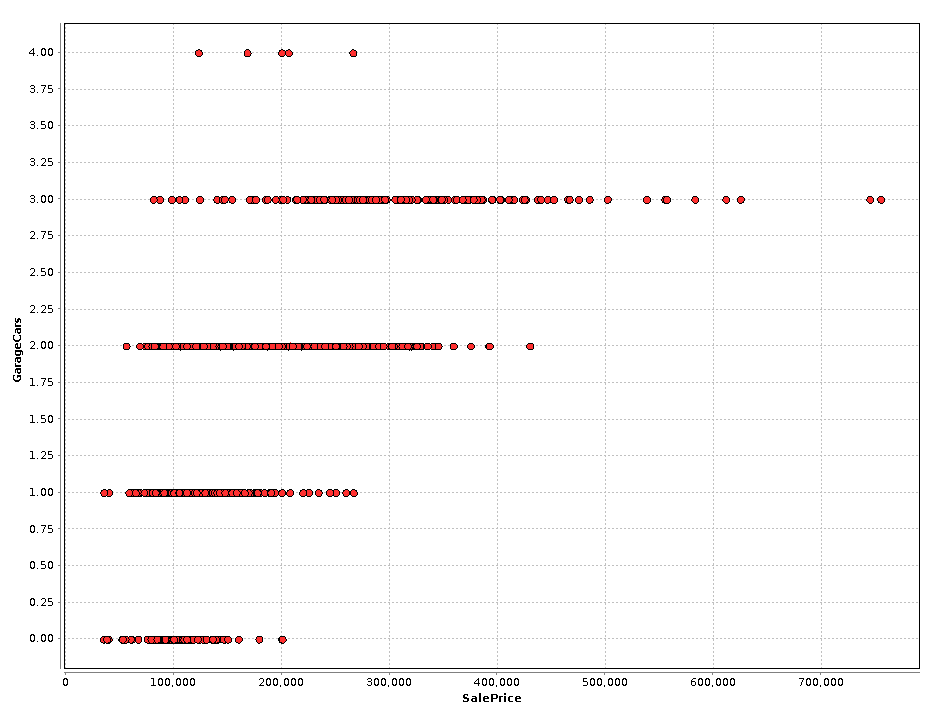
\includegraphics[width=0.7\textwidth]{GarageCars.png}
  \caption{Scatter-Plot von der Korrelation von SalePrice
  und GarageCars.}
  \label{fig:3}
\end{figure}

\FloatBarrier
\subsection{b)}
\label{subsec:a1b}

Nun wird eine lineare Regression zwischen dem Attribut OverallQual
und dem Attribut SalePrice durchgeführt zu sehen in der Abbildung
\ref{fig:linreg}.
\FloatBarrier


\begin{figure}
  \centering
  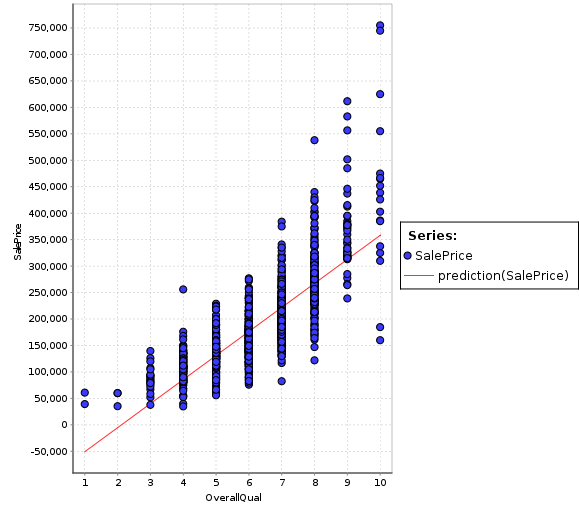
\includegraphics[width=0.7\textwidth]{Aufgabe_b.png}
  \caption{Linerare Regression zwischen SalePrice und OverallQual.}
  \label{fig:linreg}
\end{figure}

\FloatBarrier

\subsection{c)}
\label{subsec:a1c}
In der Abbildung \ref{fig:hist} wird der Relative Abstand zwischen dem geschätzten Verkaufspreisen aus
der lineraren Regression aus \ref{subsec:a1b} und den wahren Verkaufspreisen in einem
Histogramm aufgetragen.

\FloatBarrier

\begin{figure}
  \centering
  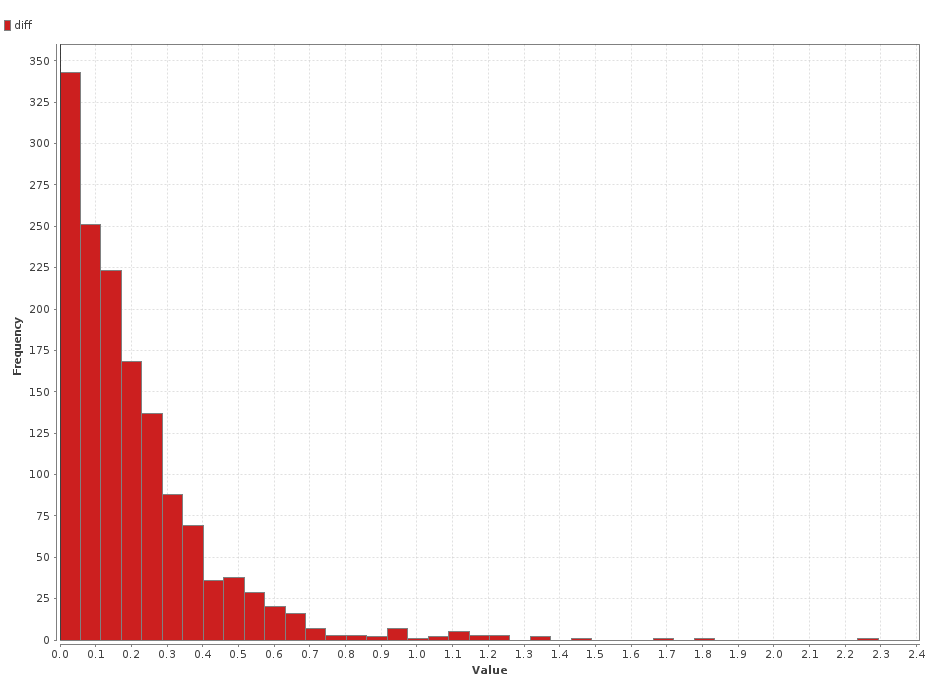
\includegraphics[width=0.7\textwidth]{histogramm.png}
  \caption{Histogramm für den Relativen Abstand von den geschätzten Verkaufspreisen
  zu den Wahren Verkaufspreisen.}
  \label{fig:hist}
\end{figure}

\FloatBarrier



\subsection{d)}
\label{subsec:a1d}
Die Aufgabe der Data-Mining-Challenge wurde mit \textbf{RapidMiner} bearbeitet.
Die zugehörigen Prozesse(als Prozessdateien und Screenshots) sowie auch die \textbf{prediction.csv}, in der das Ergebnis der
Regression zu finden ist, befinden sich im Ordner \textbf{MiningChallenge}.


Die Ergebnisse der Validierung werden beim Ausführen als \textbf{RESULT} ausgegben.
